\documentclass[conference]{IEEEtran}
\IEEEoverridecommandlockouts
\usepackage{cite}
\usepackage{amsmath,amssymb,amsfonts}
\usepackage{algorithmic}
\usepackage{mathpazo}
\usepackage[spanish]{babel}
\usepackage[utf8]{inputenc}
\usepackage[T1]{fontenc}
\usepackage{graphicx}
\usepackage{textcomp}
\usepackage{xcolor}
%\usepackage{minted}
%\usemintedstyle{emacs}
\usepackage{listings}
\lstset{language=SQL,morekeywords={PREFIX,java,rdf,rdfs,url}}
\usepackage{url}
\usepackage{ctable}
\usepackage{float}
\usepackage{amsmath,amssymb,amsfonts}
\usepackage{makecell}
\usepackage{hyperref}
\usepackage{comment}
\hypersetup{
	colorlinks=true,
	linkcolor=blue,
	filecolor=magenta,      
	urlcolor=cyan,
}
\newcommand{\DNoise}{n_d}

\newcommand{\Est}[1]{\hat{#1}}
\newcommand{\Test}[1]{\expandafter\hat#1}

\def\BibTeX{{\rm B\kern-.05em{\sc i\kern-.025em b}\kern-.08em
    T\kern-.1667em\lower.7ex\hbox{E}\kern-.125emX}}
    
\begin{document}
\title{\bf{Consultas SparQL para el filtrado de información mediante Twinkle sobre una estructura RDF extraída de la Wikidata. }}

\begin{comment}
\author{\IEEEauthorblockN{Asmat Franco, Bryan}
\IEEEauthorblockA{\textit{Universidad Nacional de Ingeniería} \\
Lima, Perú \\
\texttt{basmatf@uni.pe}}
\and
\IEEEauthorblockN{Blas Salas, Israel}
\IEEEauthorblockA{\textit{Universidad Nacional de Ingeniería} \\
Lima, Perú \\
\texttt{iblass@uni.pe}}
\and
\IEEEauthorblockN{Chavez Bruno, Victor}
\IEEEauthorblockA{\textit{Universidad Nacional de Ingeniería} \\
Lima, Perú \\
\texttt{vchavezb@uni.pe}}
\and
\IEEEauthorblockN{Guadalupe Quispe, William}
\IEEEauthorblockA{\textit{Universidad Nacional de Ingenieri\'a} \\
Lima, Perú \\
\texttt{wguadalupeq@uni.pe}}
}
\end{comment}
\author{%x  x
\textsc{Bryan Asmat}\textsc{, Danilo Blas}\textsc{, Victor Chavez}\textsc{, William Guadalupe}\\
%\thanks{A thank you or further information} \\[1ex] % Your name
\normalsize Universidad Nacional de Ingeniería \\ % Your institution
\normalsize Lima,Perú \\ % Your institution
\normalsize \href{mailto:basmatf@uni.pe}{basmatf@uni.pe},  \href{mailto:iblass@uni.pe}{iblass@uni.pe} \href{mailto:vchavezb@uni.pe}{,  vchavezb@uni.pe} \href{mailto:wguadalupeq@uni.pe}{,  wguadalupeq@uni.pe} % Your email address
%\and % Uncomment if 2 authors are required, duplicate these 4 lines if more
%\textsc{Jane Smith}\thanks{Corresponding author} \\[1ex] % Second author's name
%\normalsize University of Utah \\ % Second author's institution
%\normalsize \href{mailto:jane@smith.com}{jane@smith.com} % Second author's email address
}





\maketitle

\begin{abstract}
En el presente trabajo se implementaron consultas de tipos SparQL que permiten hacer la búsqueda en distintas fuentes de datos como estructuras RDF,la creación de esta estructura, asi como un resumen de los pasos que realizamos para la ejecución del proyecto.

Para iniciar el proyecto se usó la base de conocimiento de la Wikidata realizando consultas online \textbf{https://query.wikidata.org/} con lo cual seguiremos los siguientes pasos para que se entienda como se ha creado la estructura RDF.
\vspace{0.2cm}
Accedemos al enlace mencionado anteriormente.Podemos usar las consultas con extensión .rq que están almacenadas en el repositorio de este proyecto:
\vspace{0.2cm}
Si usamos el contenido del archivo onlineQuerySELECT.rq copiaremos la información y la usaremos en el servicio de consultas de la Wikidata nos devuelve la tabla que hemos construido mediante las consultas que hemos hecho.
Si usamos el contenido del archivo onlineQueryCONSTRUCT.rq copiaremos la información y la usaremos en el servicio de consultas de la Wikidata nos devuelve como serían las tripletas en una nueva estructura RDF que vamos a manejar.
\vspace{0.2cm}
Descargamos el archivo TSV detallado que se genera al usar el archivo onlineQueryCONSTRUCT.rq y lo modificamos para que tenga el formato Turtle a usar en el presente proyecto.
El archivo RDF en formato turtle una vez generado y se encuentra en el siguiente en el directorio RDF con el siguiente nombre RDF.ttl.
\vspace{0.2cm}
Hasta ahora los pasos que hemos hecho es para extraer una estructura RDF nueva de Wikidata realizado consultas SparQL para obtener datos de investigaciones y trabajos científicos, digamos obras, que se basen sobre el tema de Ciencias de la Computación. De estos datos hemos extraído las siguiente características:

Titulo,Autor,Tema, Idioma, Revista,  Fecha de Publicación, URL.

\vspace{0.2cm}


\end{abstract}

\section{Introducci\'on}
\vspace{0.2cm}
La información en la web se puede representar bajo un formato de datos llamado RDF.
El consorcio World Wide Web (W3C) propuso una especificación llamada SparQL(lenguaje de consultas) para manipular grafos compuestos por tripletas RDF en la web y en repositorios de datos, así como extraer datos mediante consultas a relaciones desconocidas  y realizar búsquedas con combinaciones complejas de base de datos.

\vspace{0.5cm}
La estructura de los resultados de una consulta SPARQL es una tabla donde cada fila es un resultado y cada columna se corresponde con una de las variables de la consulta.

Una consulta SparQL consta de tres partes:
\begin{itemize}
    \item  Coincidencia de patrones: optional, union, nesting,filtering.
    \item  Modificadores de solución: projection, distinct, order, límit, offset.
    \item  Parte de salida: construcción de nuevas tripletas.
\end{itemize}

\vspace{0.5cm}
Las búsquedas se realizan a través de un SparQL Endpoint, que es la interfaz de entrada y salida de estas bases de datos y que permitirá nuestras consultas. Dicho de otra forma, los Endpoints de SparQL no son más que una dirección web (URL) que acepta peticiones de búsqueda SparQL y devuelve resultados, las formas de consulta SparQL son select, construct, ask y describe.

\vspace{0.5cm}
\textbf{¿Cuáles son los desafíos de diseño en SparQL?}
\vspace{0.5cm}

SparQL debe tener en cuenta las características distintivas de RDF:
\begin{itemize}
    \item Debería poder extraer información de grafos RDF interconectados.
    \item Debe ser coherente con la semántica de mundo abierto de RDF.
    \item Debe ofrecer la posibilidad de agregar información opcional si está presente. 
    \item Debería ser capaz de interpretar correctamente grafos RDF con un vocabulario con semántica predefinida.
    \item Debería ofrecer algunas funcionalidades para navegar en un grafo RDF.
\end{itemize}

\vspace{0.2cm}

\section{¿Que es la web Semántica?}

La Web Semántica vendría a ser una extensión de la Web actual dotada de significado, esto es, un espacio donde la información tendría un significado bien definido, de manera que pudiera ser interpretada tanto por agentes humanos como por agentes computarizados.

\vspace{0.2cm}

La web Semántica ha sido impulsada, entre otros, por el creador de la web, Tim Berners Lee en el 2000 para que la información sea reunida de forma que los buscadores puedan ''comprender'', más allá de limitarse a colocar los documentos en una lista

\begin{figure}[h]
	\centering
	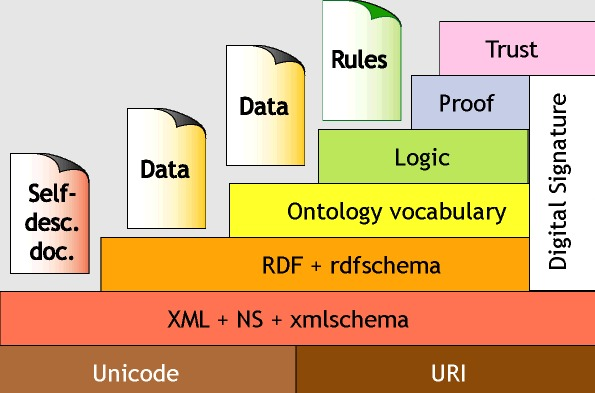
\includegraphics[scale=0.40]{imagenes/imagen1.jpeg} 
	\caption{Web semántica \cite{b4}}
\end{figure}
\section{URLs, URIs, IRIs}
\subsection{URLs}
El LRU es una cadena de caracteres con la que se asigna una dirección única a cada uno de los recursos de información disponibles en Internet. Existe un URL único para cada página de cada uno de los documentos de la WWW

\subsection{URIs}
Un identificador de recursos uniforme es una cadena de caracteres que identifica los recursos de una red de forma unívoca. La diferencia respecto a un localizador de recursos uniforme (URL) es que estos últimos hacen referencia a recursos que, de forma general, pueden variar en el tiempo. 

Normalmente estos recursos son accesibles en una red o sistema. Los URI pueden ser localizador de recursos uniforme (URL),(URN)
\subsection{IRIs}
Es un estándar de protocolo de Internet que se basa en el protocolo Identificador uniforme de recursos (URI) al expandir en gran medida el conjunto de caracteres permitidos.

\section{Estructura RDF}
RDF es un método general para descomponer cualquier tipo de conocimiento en trozos pequeños, con algunas reglas acerca de la semántica o significado, de esas piezas.

El punto es tener un método tan simple que puede expresar cualquier hecho, y a la vez tan estructurada que las aplicaciones informáticas pueden hacer cosas útiles con él.  \cite{b5}

RDF representa la información en una declaración triple -también llamada tripleta- que sigue la estructura sujeto-predicado-objeto \cite{b5}

\vspace{0.2cm}
\textbf{Ejemplo}

<La ronda de noche> <fue creada por> <Rembrandt>
\vspace{0.2cm}
En este ejemplo\textbf{<La ronda de noche>} y el objeto \textbf{<Rembrandt>} se pueden considerar como dos nodos en un grafo donde el predicado \textbf{<fue creada por>} define una arista o la relación entre estos . \cite{b5}

\vspace{0.2cm}


\section{Buscando RDF con SPARQL}
SPARQL nos permite traducir datos en grafo, intensamente enlazados, en datos normalizados en formato tabular, esto es, distribuidos en filas y columnas, que se pueden abrir  en formato como .csv .json .ttl ,etc o también se pueden ver en programas de visualización


Resulta útil pensar las consultas SPARQL como un conjunto de oraciones con espacios en blanco. La base de datos tomará esta consulta y encontrará cada conjunto de oraciones que encaje correctamente en estos espacios en blanco, devolviéndonos los valores coincidentes como una tabla.
\vspace{0.2cm}




\section{Consultas SPARQL}


SPARQL, acrónimo de SPARQL \textit{Protocol and RDF Query Language}, es un lenguaje estandarizado para hacer consultas en estructuras RDF.  Es una tecnología clave en el desarrollo de la web semántica que se constituyó como recomendación oficial del W3C el 15 de enero de 2008, siendo actualizado a la versión 1.1 en 2013\cite{b1}. En un principio SPARQL únicamente incorpora funciones para la recuperación sentencias RDF. Sin embargo, algunas propuestas también incluyen operaciones para el mantenimiento (creación, modificación y borrado) de datos.

\subsection{Especificaciones}

\textbf{SPARQL 1.0:}

\begin{itemize}
	\item SPARQL como lenguaje de consultas para RDF, cubre la sintaxis de las consultas (QL).
	\item SPARQL como protocolo para RDF especifica cómo un programa debe pasar consultas SPARQL a un servicio de procesamiento de consultas SPARQL y cómo este servicio las retorna. 
	\item Formato XML de resultados de consultas SPARQL, describe un formato simple XML para que los procesadores de consultas lo utilicen al devolver resultados.
	
\end{itemize}
\newpage
\textbf{Sparql 1.1:}
\begin{itemize}
	\item La especificación de consulta federada describe como una simple consulta puede traer data de multiples fuentes, esto hace más fácil construir aplicaciones que toman ventaja de entornos distribuidos.
	\item La especificación de actualización es la diferencia clave entre SPARQL 1.0 y 1.1 porque lleva a SPARQL de ser un lenguaje de consulta a algo que puede agregar datos a un conjunto de datos, reemplazarlos y eliminarlos también.
	\item La especificación de Descripción del servicio describe cómo un programa cliente puede preguntarle a un motor SPARQL exactamente qué características admite.
	\item La especificación del formato JSON de los resultados de la consulta describe un equivalente JSON del formato XML de los resultados de la consulta.
	\item La especificación de los formatos CSV y TSV de los resultados de la consulta describe los equivalentes de valores separados por comas y tabuladores del formato XML de los resultados de la consulta.
	\item La especificación del Protocolo HTTP de Graph Store amplía el Protocolo SPARQL con una API similar a REST para la comunicación entre un cliente y un procesador SPARQL sobre gráficos o conjuntos de tripletas.  \cite{b4}
	
\end{itemize}

\subsection{Ejemplos de Consultas}
Veamos algunas consultas que son comunes y así poder entenderlas.

\textbf{Ejemplo}
\begin{lstlisting}[captionpos=b, caption=SPARQL query, label=lst:sparql,
basicstyle=\ttfamily,frame=single]
SELECT ?subject ?predicate ?object
WHERE {
	?subject ?predicate ?object .
}
\end{lstlisting}


En esta consulta, seleccionamos todas las variables del patrón para poder representarlas con un *carácter. Además, las variables se pueden llamar de cualquier manera.

Obviamente, para obtener consultas mas útiles, se deberá corregir las variables . Cambiando el predicado podemos obtener veinte entidades con sus etiquetas:


\begin{lstlisting}[captionpos=b, caption=SPARQL query, label=lst:sparql,
basicstyle=\ttfamily,frame=single]
PREFIX wdt: <http://www.wikidata.org/prop/
direct/> 
SELECT *
WHERE {
?obra wdt:titulo ?titulo . 
}
LIMIT 10
\end{lstlisting}
Si se desea revisar mas ejemplos de consultas revisar el siguiente enlace
\cite{b7}
\newpage
\subsection{Estructura RDF a utilizar}

\begin{figure}[h]
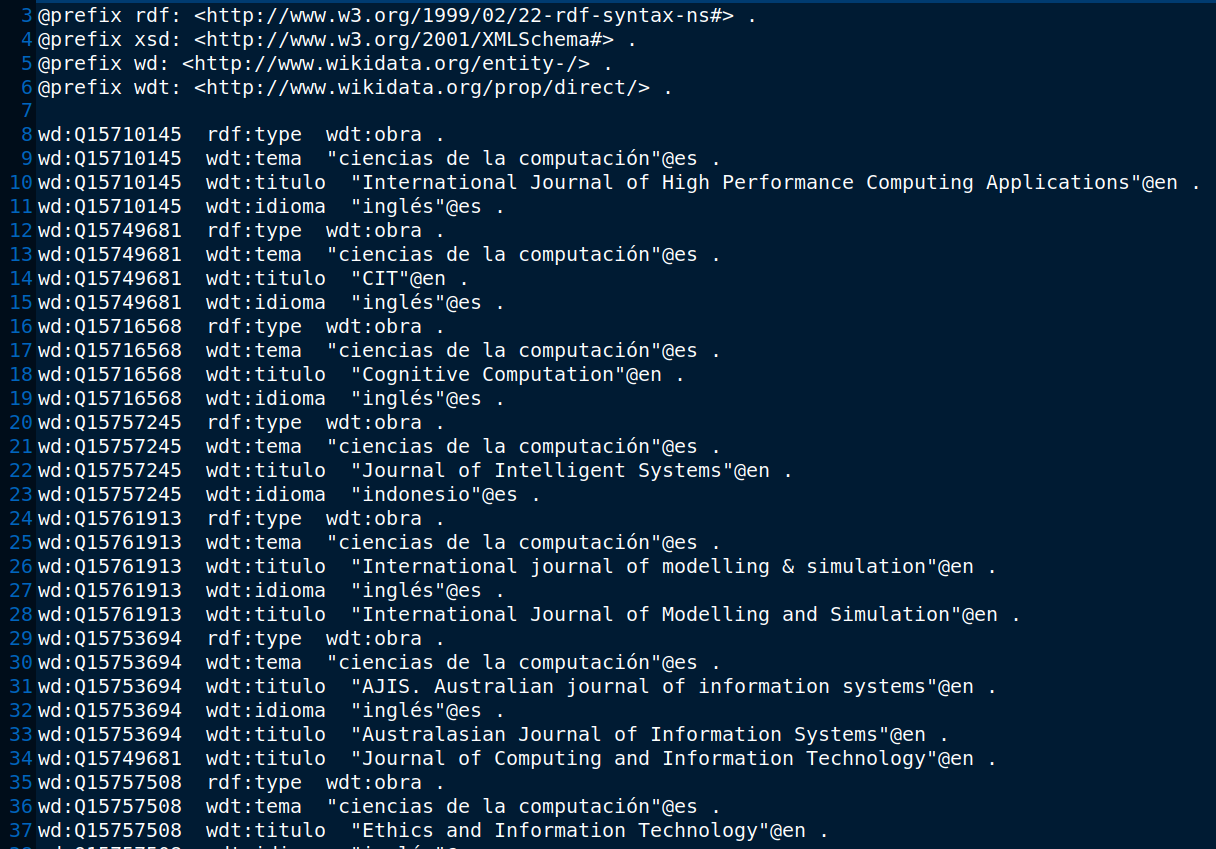
\includegraphics[scale=0.2]{imagenes/estruc_rdf_30.png} 
\caption{30 tripletas de la estructura RDF utilizada (ver archivo RDF.ttl) }
\end{figure} 

\begin{figure}[h]
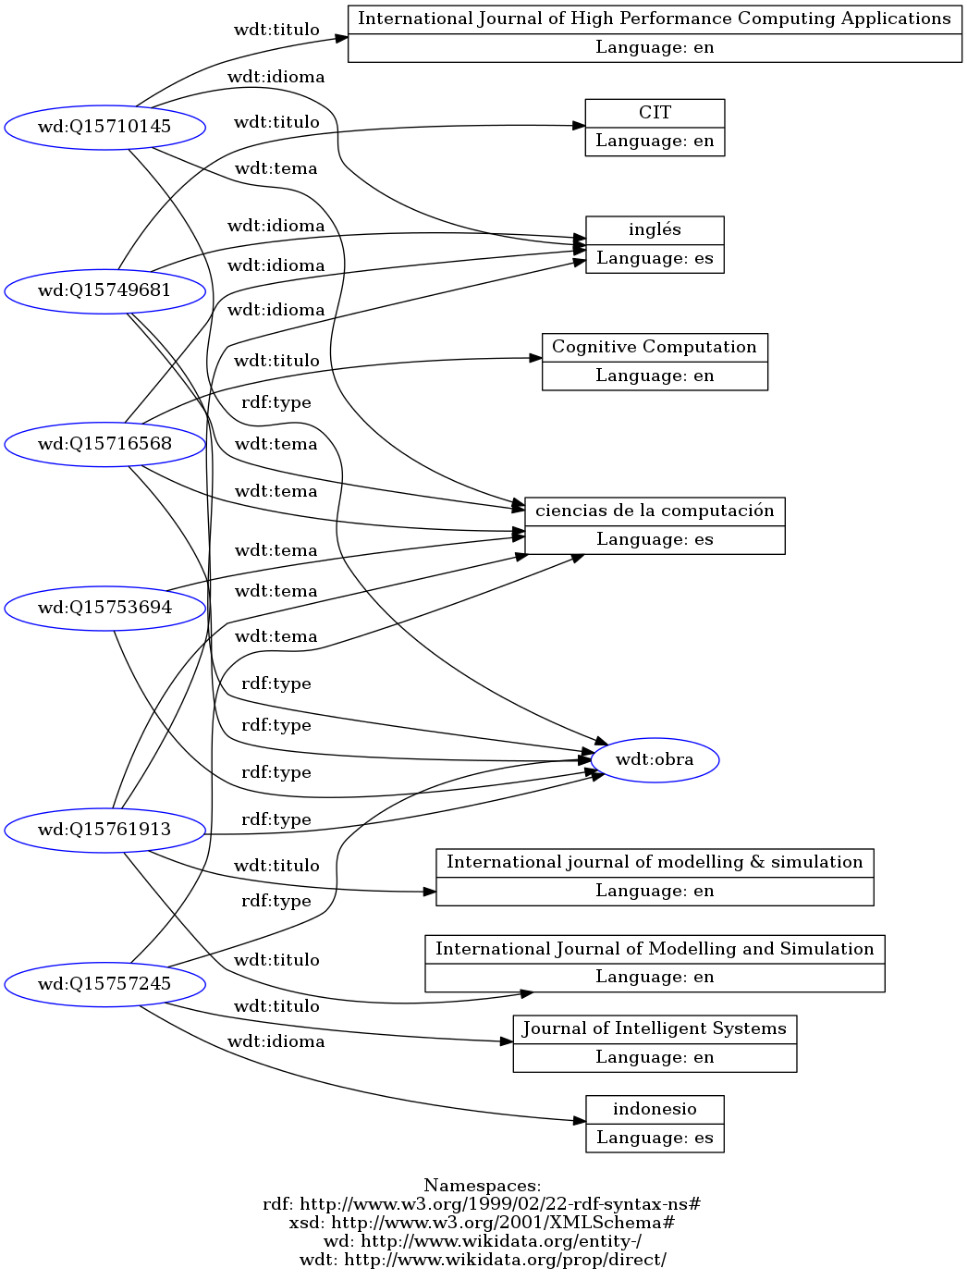
\includegraphics[scale=0.25]{imagenes/grafo_rdf_30.jpeg} 
\caption{Grafo generado con 30 tripletas de la estructura RDF utilizada \cite{b2}}
\end{figure} 

\vspace{0.2cm}

Como podemos Apreciar en la figura anterior es muestra la data ya lista para usarse y pasare a explicar algunas lineas y sea mas fácil para los usuarios que vienen a ser abreviaturas de prefijos para WikiData que es donde hemos bajado la información
\begin{itemize}
	\item \textbf{wd: } Una entidad de WikiData como se puede apreciar en el URL  <http://www.wikidata.org/entity/>
	\item \textbf{wdt: } Propiedades de una entidad de WikiData  <http://www.wikidata.org/prop/direct/>
	\item \textbf{@en:} Nos dice en que idioma esta  en este caso \textit{English} y así sucesivamente si en caso fuera \textbf{@es} el idioma español
	\item\textbf{type:}Es una instancia de una clase
\end{itemize}

\newpage

\section{Conclusiones}

\begin{itemize}
\item  SPARQL es un lenguaje bastante flexible e intuitivo de aprender , dando nos la facilidad de poder realizar consultas complejas. 
\item Después extracción de datos en WikiData, estos deben ser limpiados y dar formato \textit{turtle} para así poder realizar consultas en Twinkle.
\item Es mejor trabajar con los servicios  de consultas en linea por la mayor capacidad de data que tienen y por la mayor funcionalidad que tienen para realizar consultas.

\end{itemize}

%\section{Referencias}
\begin{thebibliography}{00}
\bibitem{b1}\href{https://arxiv.org/abs/1502.03167}{https://www.w3.org/TR/rdf-sparql-query/}. 
\bibitem{b2}Página web para generar grafos a partir de una estructura RDF: \href{https://www.ldf.fi/service/rdf-grapher}{https://www.ldf.fi/service/rdf-grapher}.
\bibitem{b3} Jimmy Lei Ba, Jamie Ryan Kiros, Geoffrey E.Hinton. Layer Normalization (2016). Disponible en \href{https://arxiv.org/abs/1607.06450}{https://arxiv.org/abs/1607.06450}.
\bibitem{b4}Learning SPARQL
Querying and Updating with SPARQL 1.1
\bibitem{b5}Uso de SPARQL para acceder a datos abiertos enlazados \href{https://programminghistorian.org/es/lecciones/retirada/sparql-datos-abiertos-enlazados}{https://programminghistorian.org/es/lecciones/retirada/sparql-datos-abiertos-enlazados}

\bibitem{b6}{SPARQL query}
\href{https://medium.com/wallscope/constructing-sparql-queries-ca63b8b9ac02}{https://medium.com/wallscope/constructing-sparql-queries-ca63b8b9ac02}

\bibitem{b7}{Consultas SparQL Github}

\href{https://github.com/wguadalupeq/practicaSparQL/tree/main/RDF}{https://github.com/wguadalupeq/practicaSparQL/tree/main/RDF}

\end{thebibliography}

\end{document}